\documentclass[11pt]{article}

\usepackage[a4paper,margin=2.5cm]{geometry}
\usepackage[T1]{fontenc}
\usepackage[utf8]{inputenc}
\usepackage{amsmath,amssymb}
\usepackage{graphicx}
\usepackage{booktabs}
\usepackage{longtable}
\usepackage{array}
\usepackage{hyperref}
\usepackage{enumitem}
\usepackage{xcolor}
\usepackage{caption}
\usepackage{microtype}
\usepackage{tikz}
\usetikzlibrary{arrows.meta,positioning,shapes.geometric,fit}
\urlstyle{tt}

\graphicspath{{reports/figures/}{figures/}}
\setlist[itemize]{leftmargin=1.2em}
\setlist[enumerate]{leftmargin=1.4em}
\renewcommand{\arraystretch}{1.15}
\sloppy

\newcommand{\boamp}{\textsc{boamp}}
\newcommand{\siret}{\textsc{siret}}
\newcommand{\siren}{\textsc{siren}}
\newcommand{\cpv}{\textsc{cpv}}
\newcommand{\wmae}{\textsc{wmae}}
\newcommand{\tvd}{\textsc{tvd}}
\newcommand{\pp}{\mathrm{pp}}
\newcommand{\clip}{\operatorname{clip}}
\newcommand{\ind}{\mathbb{1}}

\title{Synthetic BOAMP Benchmark for Renewal-Linkage Evaluation\\
\large Latent-Truth Generator, Conditional Fidelity Validation, Temporal and Candidate-Environment Readiness}
\author{Gigalis Predictive-Modeling Internship --- Current Independent Study}
\date{Repository state: July 2026; benchmark version \texttt{v0\_3\_temporal\_candidate\_revision}}

\begin{document}
\maketitle

\begin{abstract}
This report documents the synthetic \boamp{} benchmark now used to evaluate procurement-renewal linkage algorithms when legal ground-truth renewal labels are unavailable in the real \boamp{} corpus. The benchmark is not a substitute for the original dataset. Its purpose is narrower and more defensible: it creates a controlled world with hidden recurrence truth, corrupts the observable fields to resemble real \boamp{} notices, and then validates whether the resulting observed synthetic data is realistic enough for testing candidate generation and linkage behavior.

The current benchmark version, \texttt{v0\_3\_temporal\_candidate\_revision}, passes the readiness gates required before running linkage algorithms. Conditional field fidelity remains passing after the v0.2 revision; temporal fidelity passes at the publication-year, schema-year, notice-type-year, and 12/24-month follow-up levels; the Layer-1 production candidate environment now passes after the v0.3 revision; and structural truth checks confirm that hidden labels are internally coherent and not leaked into observed notices. The candidate environment improved from a v0.2 zero-candidate rate of 90.4\% to 63.0\%, compared with 60.9\% in the real Layer-1 source scope. The final status is \textbf{READY\_FOR\_LINKAGE}, with a documented caveat that 60-month follow-up runway remains weaker than the real corpus and that synthetic-benchmark evidence cannot replace inaccessible real truth.
\end{abstract}

\tableofcontents

\section{Technical Summary}

The practical problem is that \boamp{} notices do not contain a reliable field saying that one call for tenders is the renewal or recurrence of a previous procurement need. The production linkage algorithm must infer that relation from observable signals such as buyer identity, \cpv{} code, object text, and timing. Because the true relation is unavailable in the real dataset, algorithm evaluation needs a controlled benchmark where the true relation is known but hidden from the algorithm.

The implemented benchmark follows a \emph{latent truth plus observed corruption} design. First, a clean synthetic world is generated: buyers, establishments, procurement needs, contract cycles, notices, and true successor relations. Second, observable \boamp{} fields are corrupted or omitted according to calibrated and scenario-documented mechanisms. Third, the observed synthetic notices are validated against the real corpus, while the hidden truth table is kept separate for later algorithm evaluation.

\begin{center}
\fbox{\parbox{0.92\textwidth}{%
\textbf{Current decision.} The v0.3 central-provisional
\texttt{observed\_notices.parquet} file is ready to be used as the observed
input to the linkage algorithms. The corresponding hidden labels are in
\texttt{true\_relations.parquet}. The linkage algorithms must not read the
truth file during candidate generation, scoring, calibration, or threshold
selection.}}
\end{center}

The final benchmark is credible enough for linkage testing for four reasons.
\begin{enumerate}
    \item \textbf{Conditional fidelity passes.} The benchmark reproduces key observable conditional rates: \siret{} presence, duration presence, \cpv{} missingness, and generic or repeated text.
    \item \textbf{Temporal fidelity passes.} Publication-year composition, schema-by-year composition, notice-type-by-year composition, and 12/24-month follow-up runway match the real corpus within the defined acceptance gates.
    \item \textbf{Candidate environment passes.} The actual Layer-1 candidate generator sees a synthetic source/candidate environment close enough to the real production source scope.
    \item \textbf{Structural truth passes.} Every cycle has exactly one outgoing truth relation, observed notices contain no truth columns, synthetic identifiers are valid and non-leaking, and a meaningful broad true-gap tail remains.
\end{enumerate}

\section{Problem and Evidence Standard}

\subsection{The real-data limitation}

\boamp{} is the \emph{Bulletin Officiel des Annonces de Marches Publics}, the French public-procurement gazette. It publishes standalone notices such as \emph{appel d'offre} notices (calls for tenders) and \emph{attribution} notices (award notices). A later notice may correspond to a recurrence of an earlier procurement need, but the corpus does not provide a complete ground-truth relation table.

This creates an evaluation problem. If an algorithm links notice \(i\) to notice \(j\), the real dataset generally cannot say with certainty whether that link is correct. Manual review can help, but it is limited and expensive. The synthetic benchmark therefore provides a controlled evaluation environment:
\[
\text{known latent truth} \rightarrow \text{realistic observed corruption} \rightarrow \text{blind linkage evaluation}.
\]

The benchmark is not intended to prove real-world renewal rates. It is intended to test whether a linkage algorithm can recover known recurrence structure under observation patterns similar to the real \boamp{} data.

\subsection{Definitions of important terms}

\begin{longtable}{p{0.23\textwidth}p{0.68\textwidth}}
\caption{Technical terms used in this report.}\\
\toprule
Term & Meaning \\
\midrule
\endfirsthead
\toprule
Term & Meaning \\
\midrule
\endhead
\boamp{} & French public-procurement notice corpus. In this project, it is the real source used to calibrate observable field behavior. \\
\cpv{} & Common Procurement Vocabulary. It is a European classification code for procurement subject matter. Digital/ICT scope uses divisions 32, 35, 48, and 72. \\
\siren{} & French nine-digit organization identifier. It identifies a legal unit. \\
\siret{} & French fourteen-digit establishment identifier. It begins with the corresponding \siren{} and identifies a specific establishment. \\
Latent truth & The clean hidden synthetic world: true buyers, establishments, needs, cycles, durations, and successor relations. \\
Observed corruption & The process that transforms clean truth into observed fields with missingness, invalid identifiers, rounded duration, generic text, or name variation. \\
Candidate environment & The set of possible future notices produced by the production candidate generator for each source notice. It is evaluated before scoring. \\
Zero-candidate rate & The share of eligible source notices for which the candidate generator finds no candidate. \\
Percentile / p90 & The 90th percentile. If p90 candidate count is 6, then 90\% of sources have at most 6 candidates. \\
\wmae{} & Weighted mean absolute error. It measures average absolute real-versus-synthetic error while weighting each cell by the real cell size. \\
\tvd{} & Total variation distance. It measures the distance between two discrete distributions. \\
Structural truth & Internal validity of hidden labels: one outgoing relation per cycle, no duplicated successor target where forbidden, no truth leakage into observed data. \\
Truth leakage & A failure mode where fields such as \texttt{cycle\_id\_true} or \texttt{need\_id\_true} appear in the observed data used by the algorithm. \\
\bottomrule
\end{longtable}

\section{Benchmark Data Scope and Artifacts}

\subsection{Real \boamp{} dataset used as the observable reference}

The real reference dataset is \texttt{data/interim/boamp\_common\_prepared.csv}.
It is a prepared \boamp{} analysis table, not a truth-labeled renewal table. It
contains 84,623 notices and 94 columns covering publications from 2 March 2015
to 13 July 2026. The table is used to calibrate and validate observable
structure: which fields are present, how notice types and schemas evolve over
time, how buyer identifiers appear or disappear, how \cpv{} codes are
distributed, and how text and duration fields behave.

\begin{table}[h!]
\centering
\caption{Real prepared \boamp{} corpus profile. Percentages are computed over 84,623 records in \texttt{boamp\_common\_prepared.csv}.}
\begin{tabular}{lr}
\toprule
Quantity & Value \\
\midrule
Records & 84,623 \\
Columns & 94 \\
Publication period & 2015-03-02 to 2026-07-13 \\
Notice types & 58,292 calls; 22,560 awards; 3,771 other \\
Schema families & 73,941 legacy; 10,682 eForms \\
Distinct buyer keys & 5,268 \\
Distinct cleaned \siret{} values & 1,689 \\
Distinct cleaned \siren{} values & 1,506 \\
Distinct cleaned \cpv{} codes & 3,145 \\
Distinct \cpv{} divisions & 45 \\
Distinct normalized object texts & 58,918 \\
\bottomrule
\end{tabular}
\end{table}

The main field groups are:
\begin{itemize}
    \item \textbf{Notice identity and dates:} \texttt{notice\_id}, \texttt{publication\_date}, \texttt{publication\_year}, \texttt{publication\_month}, end-diffusion fields, and linked-attribution dates where available.
    \item \textbf{Notice type and schema:} \texttt{notice\_type\_normalized} and \texttt{schema\_family}; these distinguish calls for tenders, awards, legacy notices, and eForms notices.
    \item \textbf{Buyer identifiers:} raw and cleaned \siret{}/\siren{} candidates, identifier validity flags, \texttt{buyer\_key}, \texttt{buyer\_key\_type}, buyer name fields, and buyer identity layer.
    \item \textbf{\cpv{} fields:} raw and cleaned \cpv{} values, \cpv{} division/group/class/category fields, \texttt{cpv\_missing}, generic-\cpv{} flags, and digital-scope indicators.
    \item \textbf{Text fields:} raw, cleaned, and normalized object text fields such as \texttt{objet\_clean}, \texttt{objet\_normalized}, and \texttt{text\_length}.
    \item \textbf{Dates and durations:} raw duration extraction, declared duration in months, duration unit, validity flag, quality flag, and imputation indicator.
\end{itemize}

The important missingness pattern is not an error in the prepared data; it is
part of the real observation environment that the synthetic benchmark must
reproduce. Cleaned \siret{} and \siren{} are missing for 72.78\% of notices,
\cpv{} is missing for 17.06\%, raw duration is missing for 86.35\%, and
declared duration in months is missing for 83.20\%. Buyer names, notice type,
schema family, and publication date are effectively complete in the prepared
corpus. This explains why the benchmark validation focuses on conditional
field availability rather than expecting all fields to be complete.

\subsection{Exact benchmark objective}

The objective is to build a synthetic benchmark that approximates the
observable structure and linkage difficulty of the real \boamp{} corpus while
retaining hidden truth labels for evaluation. The benchmark therefore has
three explicit constraints:
\begin{enumerate}
    \item it does not replace real ground truth, because real legal renewal
    labels are not available at corpus scale;
    \item it should resemble the real data in the fields that a linkage
    algorithm actually observes: buyer identity, \cpv{}, text, dates,
    duration availability, temporal runway, and candidate availability;
    \item it will be used to compare procurement-linkage algorithms only after
    the algorithm has produced predictions without reading hidden truth files.
\end{enumerate}

\subsection{Current benchmark version}

The active benchmark version is \texttt{v0\_3\_temporal\_candidate\_revision}. It keeps the v0.2 conditional-field improvements and adds a temporal/candidate-environment revision targeted at the actual Layer-1 source scope. The benchmark was generated with fixed seeds:
\[
\text{latent world seed}=20260721,\qquad \text{corruption seed}=20260722.
\]

\begin{table}[h!]
\centering
\caption{Generated v0.3 central-provisional row counts. Counts come from \texttt{generation\_metadata.json}.}
\begin{tabular}{lr}
\toprule
Table & Rows \\
\midrule
Latent buyers & 2,000 \\
Latent establishments & 2,174 \\
Latent procurement needs & 4,800 \\
Latent cycles & 6,866 \\
True relations & 6,866 \\
Notice-family membership & 9,471 \\
Clean notices & 9,471 \\
Observed notices & 9,471 \\
Corruption log & 32,344 \\
\bottomrule
\end{tabular}
\end{table}

\subsection{Files to use for linkage evaluation}

The synthetic benchmark deliberately separates algorithm-facing observations
from hidden truth and generator internals. This is why the synthetic observed
dataset has fewer columns than the real prepared dataset: the observed file is
the restricted input that a linkage algorithm may read, whereas the real
prepared file contains many helper columns created during cleaning and
diagnostics.

\begin{longtable}{p{0.29\textwidth}p{0.60\textwidth}}
\caption{Primary v0.3 artifacts.}\\
\toprule
Artifact & Role \\
\midrule
\endfirsthead
\toprule
Artifact & Role \\
\midrule
\endhead
\texttt{observed notices} & The observed synthetic notice table, stored as \nolinkurl{observed_notices.parquet}. This is the input that linkage algorithms may read. \\
\texttt{latent buyers, establishments, needs, cycles} & Hidden entity and contract-cycle tables, stored in \nolinkurl{latent_buyers.parquet}, \nolinkurl{latent_establishments.parquet}, \nolinkurl{latent_needs.parquet}, and \nolinkurl{latent_cycles.parquet}. These contain the clean synthetic world and must not be used by linkage algorithms. \\
\texttt{true relations} & Hidden true links, stored as \nolinkurl{true_relations.parquet}. Each source cycle has one outgoing relation: \texttt{NEXT\_CYCLE} when a true successor exists or \texttt{NO\_SUCCESSOR} otherwise. This file must be used only after algorithm outputs are produced. \\
\texttt{clean notices} & Pre-corruption notice records, stored as \nolinkurl{clean_notices.parquet}. These preserve clean generator state and are not algorithm input. \\
\texttt{corruption log} & Audit trail showing how clean fields were corrupted into observed fields. It is for generator validation, not linkage input. \\
\texttt{generation metadata} & Generator version, seeds, config hashes, row counts, selected v0.3 candidate-revision parameters, and validation status. \\
\texttt{conditional observation parameters} & Smoothed conditional field-availability probabilities used by the v0.2 observation revision. \\
\texttt{selected params} & Parameter-provenance CSV for the v0.3 temporal/candidate revision. \\
\bottomrule
\end{longtable}

\section{End-to-End Generator Pipeline}

\subsection{Flowchart}

\begin{figure}[p]
\centering
\resizebox{\textwidth}{!}{%
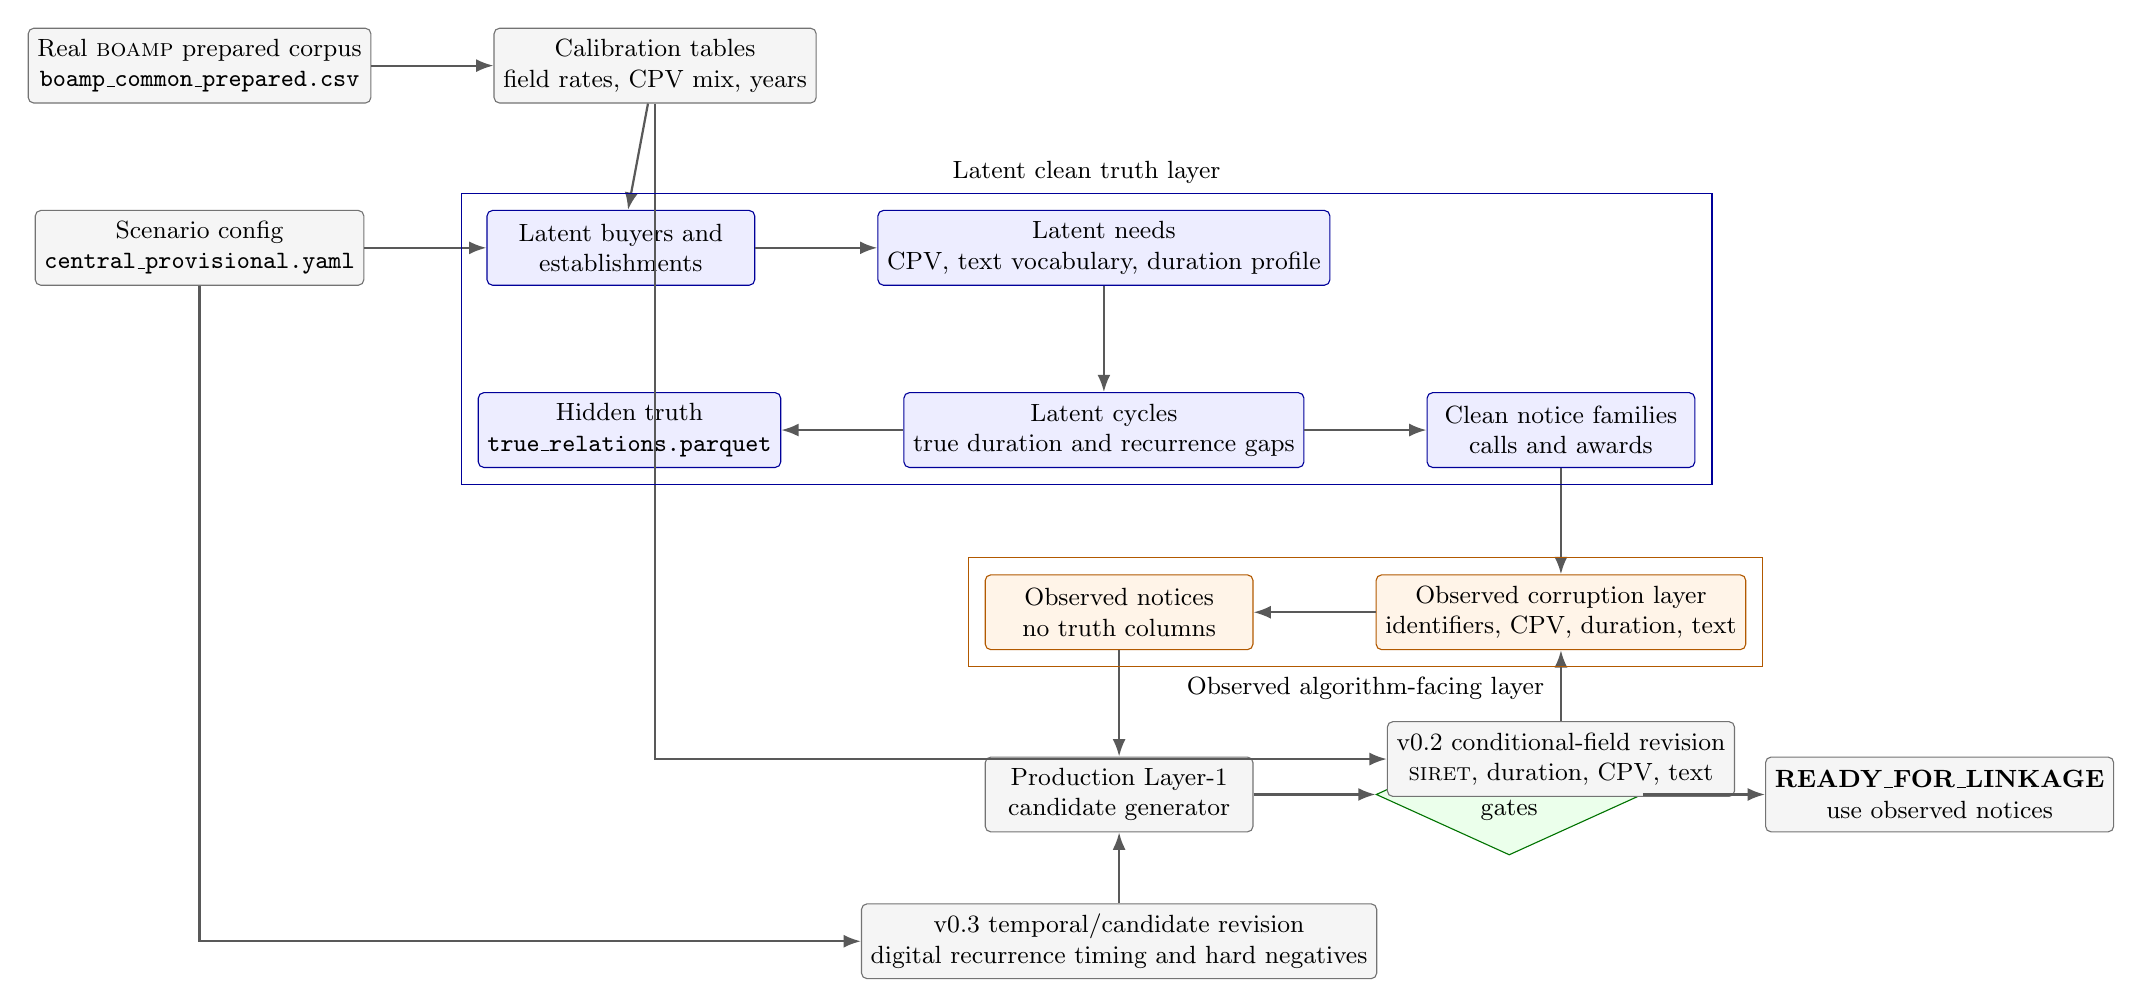
\begin{tikzpicture}[
    node distance=1.35cm and 1.55cm,
    block/.style={rectangle, rounded corners=2pt, draw=black!55, fill=gray!8, align=center, minimum width=3.4cm, minimum height=0.95cm, font=\small},
    truth/.style={rectangle, rounded corners=2pt, draw=blue!60!black, fill=blue!7, align=center, minimum width=3.4cm, minimum height=0.95cm, font=\small},
    obs/.style={rectangle, rounded corners=2pt, draw=orange!70!black, fill=orange!9, align=center, minimum width=3.4cm, minimum height=0.95cm, font=\small},
    gate/.style={diamond, aspect=2.2, draw=green!45!black, fill=green!8, align=center, font=\small, inner sep=2pt},
    arrow/.style={-{Latex[length=2.2mm]}, thick, draw=black!65}
]
\node[block] (real) {Real \boamp{} prepared corpus\\ \texttt{boamp\_common\_prepared.csv}};
\node[block, right=of real] (calib) {Calibration tables\\ field rates, CPV mix, years};
\node[block, below=of real] (scenario) {Scenario config\\ \texttt{central\_provisional.yaml}};
\node[truth, right=of scenario] (buyers) {Latent buyers and\\ establishments};
\node[truth, right=of buyers] (needs) {Latent needs\\ CPV, text vocabulary, duration profile};
\node[truth, below=of needs] (cycles) {Latent cycles\\ true duration and recurrence gaps};
\node[truth, left=of cycles] (relations) {Hidden truth\\ \texttt{true\_relations.parquet}};
\node[truth, right=of cycles] (clean) {Clean notice families\\ calls and awards};
\node[obs, below=of clean] (corrupt) {Observed corruption layer\\ identifiers, CPV, duration, text};
\node[obs, left=of corrupt] (observed) {Observed notices\\ no truth columns};
\node[block, below=of observed] (candidate) {Production Layer-1\\ candidate generator};
\node[gate, right=of candidate] (valid) {Validation\\ gates};
\node[block, right=of valid] (ready) {\textbf{READY\_FOR\_LINKAGE}\\ use observed notices};

\node[block, below=0.9cm of corrupt] (v2) {v0.2 conditional-field revision\\ \(\siret\), duration, CPV, text};
\node[block, below=0.9cm of candidate] (v3) {v0.3 temporal/candidate revision\\ digital recurrence timing and hard negatives};

\draw[arrow] (real) -- (calib);
\draw[arrow] (calib) -- (buyers);
\draw[arrow] (scenario) -- (buyers);
\draw[arrow] (buyers) -- (needs);
\draw[arrow] (needs) -- (cycles);
\draw[arrow] (cycles) -- (relations);
\draw[arrow] (cycles) -- (clean);
\draw[arrow] (clean) -- (corrupt);
\draw[arrow] (corrupt) -- (observed);
\draw[arrow] (observed) -- (candidate);
\draw[arrow] (candidate) -- (valid);
\draw[arrow] (valid) -- (ready);
\draw[arrow] (v2) -- (corrupt);
\draw[arrow] (v3) -- (candidate);
\draw[arrow] (calib) |- (v2);
\draw[arrow] (scenario) |- (v3);

\node[draw=blue!60!black, fit=(buyers)(needs)(cycles)(relations)(clean), inner sep=6pt, label={[font=\small]above:Latent clean truth layer}] {};
\node[draw=orange!70!black, fit=(corrupt)(observed), inner sep=6pt, label={[font=\small]below:Observed algorithm-facing layer}] {};
\end{tikzpicture}}
\caption{End-to-end benchmark pipeline. The blue layer contains hidden truth and must not be used by the linkage algorithm. The orange layer is the observed synthetic data that mimics real \boamp{} field availability and corruption.}
\label{fig:pipeline-flowchart}
\end{figure}

\subsection{Pipeline stages}

The generator is split into two independent random streams: one for the latent clean world and one for observation/corruption. This separation lets a future experiment hold the true world fixed while changing observation corruption, or hold corruption fixed while changing latent truth assumptions.

\begin{longtable}{p{0.22\textwidth}p{0.68\textwidth}}
\caption{Generator stages and their interpretation.}\\
\toprule
Stage & Description \\
\midrule
\endfirsthead
\toprule
Stage & Description \\
\midrule
\endhead
Latent buyers & Generates synthetic public buyers with department, buyer type, synthetic organization name, \siren{}, activity rate, activity tier, active window, alias propensity, and identifier-quality propensity. Buyer activity is heavy-tailed, so concentration is emergent rather than assigned directly. \\
Latent establishments & Generates valid \siret{} values under the buyer's \siren{} hierarchy. This permits establishment-level identity errors without using real identifiers. \\
Latent needs & Generates procurement needs under each buyer: CPV code, broad segment, base text concepts, vocabulary, duration profile, and recurrence propensity. \\
Latent cycles & Generates one or more contract cycles for each need. Each cycle has a start date, true duration, expected end, and possibly a successor cycle. \\
True relations & Derives \texttt{NEXT\_CYCLE} or \texttt{NO\_SUCCESSOR} for every cycle from the latent cycle table. This is the hidden evaluation truth. \\
Clean notices & Generates an \texttt{APPEL\_OFFRE} call notice for every cycle and an \texttt{ATTRIBUTION} award notice with calibrated probability. \\
Observed corruption & Corrupts identifiers, buyer names, CPV, duration, object text, and linked-call visibility. This creates observed notices shaped like real prepared \boamp{} data. \\
Validation & Compares observed synthetic data against real data on field availability, temporal structure, candidate environment, and structural truth. \\
\bottomrule
\end{longtable}

\subsection{Concrete generation procedure}

The implemented generation process can be read as the following reproducible algorithm. This is the logic used to create the final v0.3 central-provisional dataset; row counts are emergent outputs, not manually forced row-by-row.

\begin{enumerate}
    \item \textbf{Load fixed inputs.} The run loads the benchmark defaults, the central-provisional scenario, empirical calibration tables, and the prepared real \boamp{} corpus used to estimate observable rates. The v0.3 run uses fixed seeds \(20260721\) for the latent world and \(20260722\) for corruption.
    \item \textbf{Generate buyers.} The generator samples 2,000 synthetic buyers with department, buyer type, synthetic name, \siren{}, active date window, activity rate, identifier-quality propensity, and alias propensity. No real buyer name or real identifier is copied.
    \item \textbf{Generate establishments.} For each buyer, one or more valid \siret{} establishments are created under that buyer's \siren{}. This produces a realistic \siren{}--\siret{} hierarchy before any observed identifier corruption is applied.
    \item \textbf{Generate procurement needs.} For each buyer, the number of needs is sampled from the activity-tier Poisson model. Each need receives a synthetic \cpv{} code, a CPV-conditioned text vocabulary, a duration profile, and a recurrence propensity.
    \item \textbf{Generate cycles.} Each need starts with one procurement cycle. Additional cycles are sampled from the recurrence propensity until the maximum cycle count, failed successor draw, or observation-window boundary stops the chain. The cycle table contains true start dates, true durations, and true expected end dates.
    \item \textbf{Derive hidden truth.} The truth table is derived from cycles only. If a cycle is followed by another cycle of the same need, the relation is \texttt{NEXT\_CYCLE}; otherwise it is \texttt{NO\_SUCCESSOR}. Thus every cycle has exactly one outgoing truth relation.
    \item \textbf{Generate clean notices.} Every cycle creates one call-for-tenders notice. An award notice is added with the calibrated award probability. These notices still contain clean truth fields and are not given to the linkage algorithm.
    \item \textbf{Corrupt observed fields.} Identifier, buyer-name, \cpv{}, duration, text, and linked-call visibility mechanisms transform clean notices into observed notices. The observed output uses real-pipeline-like columns and intentionally contains no truth columns.
    \item \textbf{Apply v0.3 candidate revision.} For the digital \cpv{} divisions \(32,35,48,72\), selected v0.3 settings increase the chance that future same-buyer candidates exist in the production candidate window while preserving a broad true-gap tail and relation integrity.
    \item \textbf{Write versioned outputs.} The final files are written under \texttt{v0\_3\_temporal\_candidate\_revision}; v0.2 outputs are not overwritten, so before/after comparisons remain reproducible.
\end{enumerate}

This procedure explains why the benchmark contains both \texttt{observed\_notices.parquet} and \texttt{true\_relations.parquet}. The first file is what the algorithm sees. The second file is hidden truth used only for evaluation after predictions are produced.

\section{Latent-Truth Model}

\subsection{Buyer population}

Buyer activity is sampled from a heavy-tailed Pareto distribution. If \(A_b\) is the raw activity draw for buyer \(b\), then
\[
A_b \sim \operatorname{Pareto}(1.0)+0.15,\qquad
r_b=\frac{A_b}{\sum_{b'} A_{b'}}.
\]
The normalized value \(r_b\) is an activity rate. It is not directly used as a true renewal label; it shapes how many needs and notices a buyer tends to have. The intent is to reproduce the real corpus's buyer concentration pattern without copying real buyer names or identifiers.

Each buyer also receives:
\[
q_b \sim \operatorname{Beta}(5,2),\qquad a_b\sim \operatorname{Beta}(2,5),
\]
where \(q_b\) is an identifier-quality propensity and \(a_b\) is an alias-propensity value used later by the corruption layer.

\subsection{Procurement needs}

For each buyer \(b\), the number of latent procurement needs is
\begin{equation}
N_b=\max\{1,\operatorname{Poisson}(\lambda_{\text{tier}(b)})\}.
\end{equation}
The implemented tier parameters are
\[
\lambda_{\text{21+}}=8.0,\qquad
\lambda_{\text{6-20}}=4.0,\qquad
\lambda_{\text{2-5}}=1.8,\qquad
\lambda_{\text{1}}=1.2.
\]
Each need receives a \cpv{} division sampled from the empirical real-corpus division distribution, an eight-digit synthetic \cpv{}-looking code, a broad text vocabulary, a duration profile, and a recurrence propensity.

The per-need duration profile is
\begin{equation}
D_{\text{profile}}\sim \operatorname{LogNormal}(\log 12,0.7),
\end{equation}
clipped to the project duration range where needed. This creates positive, right-skewed contract-duration tendencies rather than one fixed duration for all needs.

\subsection{Recurrence propensity}

The central provisional scenario uses a base recurrence propensity \(p_0=0.40\). This is a scenario assumption, not a real-world estimate. Each need receives multiplicative jitter
\begin{equation}
J=0.7+0.6B,\qquad B\sim \operatorname{Beta}(4,4),
\end{equation}
so the implemented recurrence probability is
\begin{equation}
p_{\text{need}}=\clip(p_0J,0,0.98).
\end{equation}
The cap at 0.98 avoids deterministic recurrence while allowing highly recurrent needs.

\subsection{Cycle duration and successor gaps}

For each realized cycle, the true duration is drawn as
\begin{equation}
D_{\text{cycle}}\sim
\clip_{[1,120]}\left\{\mathcal N(D_{\text{profile}},(0.25D_{\text{profile}})^2)\right\}.
\end{equation}
The expected true end date is the true start date plus \(D_{\text{cycle}}\) months, approximated by 30.44 days per month in implementation.

Before v0.3's scoped candidate revision, broad successor gaps used the central distribution
\begin{equation}
G_{\text{broad}}\sim \clip_{[1,\infty)}\left\{\mathcal N(18,9^2)\right\}.
\end{equation}
This distribution is deliberately not centered inside the production six-month candidate window. The reason is important: latent truth should not be tuned only to make the algorithm easy. A meaningful share of true successors must remain outside the six-month window so the benchmark can test limitations in candidate generation.

\subsection{v0.3 digital-scope recurrence timing}

The v0.3 revision added an optional scoped mechanism for the digital \cpv{} divisions used by the production source filter:
\[
\mathcal D_{\text{digital}}=\{32,35,48,72\}.
\]
For scoped digital needs, recurrence propensity is multiplied by 1.3 and capped at 0.98. When a successor gap is drawn, the selected v0.3 parameter set uses a near-window gap with probability 0.75:
\begin{equation}
G_{\text{near}}\sim \clip_{[0.1,6]}\left\{\mathcal N(2,2^2)\right\}.
\end{equation}
Otherwise the broad gap \(G_{\text{broad}}\) is used. This creates more future same-buyer candidates inside the production candidate window without forcing candidate counts directly onto rows.

The v0.3 revision also permits limited same-buyer hard-negative chain alignment at rate 0.10. This shifts whole distinct-need chains from the same buyer near a source's expected end date. Because entire chains are shifted together, within-need cycle order and truth relations remain valid. The aligned target is never the same \texttt{need\_id\_true}, so these are plausible hard negatives rather than mislabeled true successors.

\section{Observed-Corruption Model}

\subsection{Why corruption is separate from truth}

The report's central methodological distinction is:
\[
\text{latent true value} \neq \text{observed BOAMP field}.
\]
For example, every latent cycle has a true duration, but the observed \texttt{declared\_duration\_months} field may be missing, rounded, converted incorrectly, or imputed later by the compatibility adapter. This separation prevents a common modeling mistake: changing the true contract duration just to fix observed duration missingness.

\subsection{Latent quality class and co-occurring errors}

Each notice is assigned a latent quality class \(Q_i\in\{\text{HIGH},\text{MEDIUM},\text{LOW}\}\). The scenario class mix is adjusted by the buyer's identifier-quality propensity. Field corruption rates are then scaled by quality-class multipliers:
\[
m(Q_i)=
\begin{cases}
0.35, & Q_i=\text{HIGH},\\
1.00, & Q_i=\text{MEDIUM},\\
2.20, & Q_i=\text{LOW}.
\end{cases}
\]
Duration uses a flatter multiplier set \(\{0.89,1.00,1.15\}\), because real duration presence behaves more like a schema/template phenomenon than a general record-quality phenomenon. This design makes field errors co-occur on lower-quality records instead of sampling every error independently.

\subsection{Weighted categorical corruption}

Several corruption mechanisms use the same pattern. If a field has base error rates \(r_k\) for outcomes \(k\), the quality-scaled rates are
\[
w_k=\min(0.98,r_km_i),
\]
renormalized if their sum exceeds one. The remaining probability is assigned to the non-corrupted outcome:
\[
P(\text{OK})=1-\sum_k w_k.
\]
This is used for mechanisms such as old identifier corruption and \cpv{} corruption.

\subsection{Conditional field observation}

The v0.2 revision replaced mainly global field mechanisms with conditional observation targets estimated from observable real data. For a cell \(g\), such as schema family by year by notice type, the smoothed target rate is
\begin{equation}
\hat p_g=\frac{x_g+\alpha \hat p_{\text{global}}}{n_g+\alpha},\qquad \alpha=25,
\end{equation}
where \(x_g\) is the number of observed successes in the real cell, \(n_g\) is the real cell size, and \(\hat p_{\text{global}}\) is the real global rate. This is a beta-binomial style shrinkage estimator. It prevents sparse cells from being copied too noisily while preserving large-cell conditional structure.

The implemented conditional targets are:
\[
P(\siret\ \text{present}\mid \text{schema},\text{year},\text{notice type}),
\]
\[
P(\text{duration present}\mid \text{schema},\text{year},\text{notice type}),
\]
and
\[
P(\text{generic repeated text}\mid \text{notice type},\text{buyer activity tier}).
\]
\cpv{} missingness is modeled by schema and notice type and remained passing without v0.3 retuning.

\subsection{Text mechanisms}

The generator separates several text concepts that should not be collapsed:
\begin{enumerate}
    \item base procurement text generated from \cpv{}-division vocabulary;
    \item small same-cycle variation between call and award notices;
    \item next-cycle lexical drift for recurrent needs;
    \item exact cross-buyer templates;
    \item near-boilerplate text with buyer-, CPV-, date-, or department-specific tokens;
    \item weak generic procurement text.
\end{enumerate}
This distinction matters because exact duplicate text across unrelated buyers is a different challenge from realistic repeated administrative language within the same buyer or same procurement family.

\section{Validation Methodology}

\subsection{Weighted mean absolute error}

For conditional rates, the main fidelity metric is weighted mean absolute error:
\begin{equation}
\operatorname{\wmae}=
\frac{\sum_g n_g^{\text{real}}\left|\hat p_g^{\text{syn}}-\hat p_g^{\text{real}}\right|}
{\sum_g n_g^{\text{real}}}.
\end{equation}
The unit is percentage points when rates are percentages. Weighting by \(n_g^{\text{real}}\) is essential because small real cells can have noisy rates. A rare cell with 20 records should not count as much as a common cell with 10,000 records.

\subsection{Total variation distance}

For distribution comparisons such as publication-year share, the report uses total variation distance:
\begin{equation}
\operatorname{\tvd}(p,q)=\frac{1}{2}\sum_k |p_k-q_k|.
\end{equation}
A value of zero means the two discrete distributions match exactly. Larger values mean more mass would need to be moved across categories to make them match.

\subsection{Candidate-count percentiles}

If \(C_i\) is the candidate count for source notice \(i\), then the empirical \(q\)-th percentile is
\begin{equation}
P_q(C)=\inf\{c:\widehat F_C(c)\ge q\}.
\end{equation}
In plain language, p90 is the value below which 90\% of sources fall. For example, real p90 candidate count \(=6\) means that 90\% of real Layer-1 source notices have at most six candidates.

The zero-candidate rate is
\begin{equation}
z=\frac{1}{N}\sum_{i=1}^N \ind(C_i=0).
\end{equation}
This is a critical candidate-environment metric because a source with no candidate cannot be recovered by any downstream scoring model.

\subsection{Evaluation workflow}

The validation is performed in three layers before the benchmark is declared ready for linkage.

\begin{enumerate}
    \item \textbf{Conditional field validation.} The notebook compares real and synthetic conditional probabilities for \siret{} presence, duration presence, \cpv{} missingness, and repeated/generic text. It reports cell-level tables, weighted and unweighted errors, signed bias, p90 error, maximum error, and pass/fail status.
    \item \textbf{Temporal validation.} The notebook compares the calendar structure of real and synthetic notices: publication-year share, publication-month share, schema by year, notice type by year, and follow-up runway at 12, 24, 36, and 60 months.
    \item \textbf{Candidate-environment validation.} The observed synthetic notices are adapted into the same shape expected by the production Layer-1 candidate generator. The actual candidate generator is then run, and the resulting source counts, zero-candidate rate, candidate-count percentiles, cap-reached rate, and buyer-key-specific zero-candidate rates are compared with the real Layer-1 source scope.
    \item \textbf{Structural-truth validation.} The validation checks that truth labels are coherent and hidden: one outgoing relation per cycle, no truth columns in observed notices, no identifier leakage, metadata validation status \texttt{PASS}, and broad true-gap tail above the required threshold.
\end{enumerate}

The key point is that the candidate environment is evaluated through the same production candidate-generation logic used later by the linkage algorithm. Candidate counts are fidelity outcomes, not direct generator assignments. This prevents the benchmark from being tuned to make a particular scorer look good.

\begin{table}[h!]
\centering
\caption{Evaluation layers and their evidence outputs.}
\small
\begin{tabular}{p{0.24\textwidth}p{0.35\textwidth}p{0.27\textwidth}}
\toprule
Evaluation layer & Main question & Main saved evidence \\
\midrule
Conditional fidelity & Do observed fields appear with realistic conditional rates? & Conditional fidelity summary and all-cell tables. \\
Temporal fidelity & Does the synthetic corpus have realistic calendar and follow-up structure? & Temporal summary and follow-up runway tables. \\
Candidate environment & Does the production candidate generator see a realistic source/candidate universe? & Candidate environment summary and gate tables. \\
Structural truth & Is hidden truth coherent and absent from observed notices? & Temporal truth sanity checks and metadata. \\
\bottomrule
\end{tabular}
\end{table}

\section{Revision History}

\subsection{v0.1 provisional benchmark}

The v0.1 benchmark established the initial latent-truth-and-corruption architecture. It generated synthetic buyers, needs, cycles, notices, true relations, and observed corruptions. It also created initial global fidelity checks. The main limitation was that several fields matched marginal rates more than conditional structure.

\subsection{v0.2 conditional revision}

The v0.2 revision targeted conditional field fidelity. It replaced or refined mechanisms for \siret{} presence, duration presence, \cpv{} missingness, and repeated/generic text. The most important methodological improvement was moving from global field rates to smoothed conditional observation models based on observable real-data cells.

The v0.2 result passed conditional fidelity but failed the production candidate environment. In the actual Layer-1 source scope, the synthetic zero-candidate rate was 90.4\%, far above the real 60.9\%, and p90 candidates/source was 0 instead of the real value 6. This meant the benchmark was not yet ready for linkage evaluation, even though the field-level validation had improved.

\subsection{v0.3 temporal/candidate revision}

The v0.3 revision preserved v0.2 conditional fidelity and changed the latent digital recurrence/candidate environment. It did not assign candidate counts directly. It did not use linkage scores, accepted links, precision, recall, score calibration, or thresholds as generator inputs.

The bounded pilot sweep tested fixed ordered parameter sets for recurrence multiplier, near-window share, and hard-negative alignment rate. The first passing setting was:
\begin{align*}
\text{recurrence multiplier} &= 1.3,\\
\text{near-window share} &= 0.75,\\
\text{hard-negative alignment rate} &= 0.10.
\end{align*}
Additional selected settings were same-buyer clustering for scoped digital needs, scoped buyer affinity share 0.07, high scoped-need probability 0.70, stable scoped establishment, and stable scoped name fallback.

\section{Final Results}

\subsection{Freeze-gate status}

\begin{table}[h!]
\centering
\caption{Final v0.3 freeze gate.}
\small
\begin{tabular}{p{0.23\textwidth}p{0.20\textwidth}p{0.45\textwidth}}
\toprule
Dimension & Status & Interpretation \\
\midrule
Conditional fidelity & PASS & v0.3 remains under thresholds with no material regression versus v0.2. \\
Temporal validation & PASS & Calendar and 12/24-month follow-up gates pass. \\
Candidate environment & PASS & Production Layer-1 candidate generator passes source-scope gates. \\
Structural truth & PASS & Metadata, truth leakage, and broad-gap-tail checks pass. \\
Linkage readiness & READY FOR LINKAGE & Linkage algorithms may now be run on observed v0.3 notices. \\
\bottomrule
\end{tabular}
\end{table}

\subsection{Conditional fidelity}

\begin{table}[h!]
\centering
\caption{Conditional fidelity summary. \wmae{} values are in percentage points.}
\small
\begin{tabular}{p{0.25\textwidth}rrrr}
\toprule
Target & v0.2 \wmae{} & v0.3 \wmae{} & Regression vs v0.2 & Status \\
\midrule
\cpv{} missingness & 2.57 & 2.09 & -0.48 & PASS \\
Duration presence & 0.51 & 0.62 & +0.11 & PASS \\
Generic repeated text & 1.40 & 0.80 & -0.60 & PASS \\
\siret{} presence & 1.88 & 1.60 & -0.28 & PASS \\
\bottomrule
\end{tabular}
\end{table}

\begin{figure}[h!]
\centering
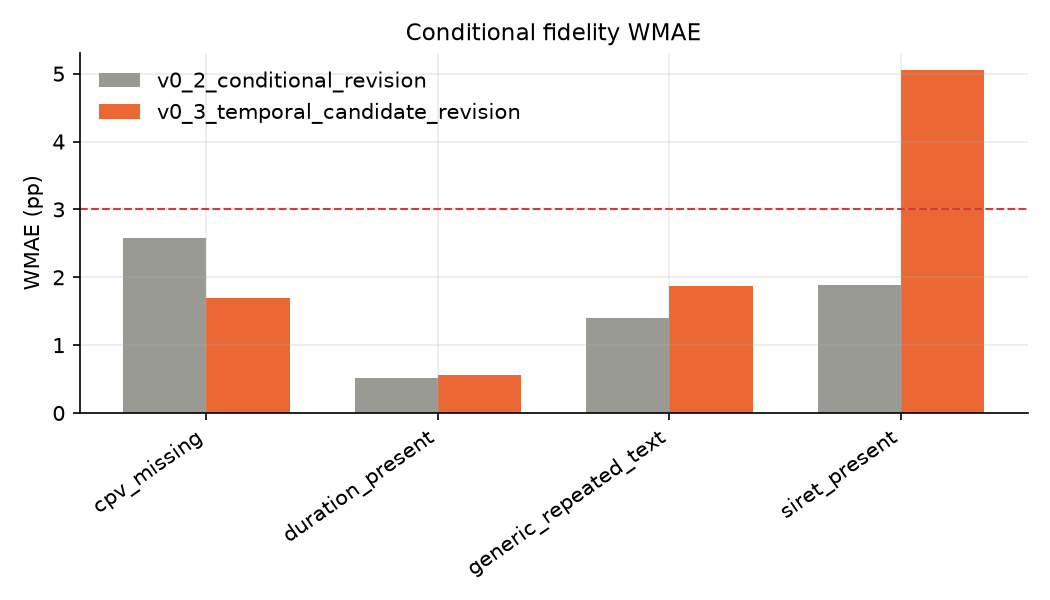
\includegraphics[width=0.86\textwidth]{synthetic_benchmark/v0_3_temporal_candidate_revision/conditional_fidelity_v0_2_v0_3_wmae.png}
\caption{Conditional-field fidelity after the v0.3 revision. The figure shows that v0.3 preserves the v0.2 conditional fixes. It supports field-fidelity readiness, but it does not by itself prove candidate-environment realism.}
\label{fig:conditional-wmae}
\end{figure}

\subsection{Temporal validation}

\begin{table}[h!]
\centering
\caption{Temporal summary metrics for v0.3.}
\begin{tabular}{llrl}
\toprule
Dimension & Metric & Value & Status \\
\midrule
Publication-year share & \tvd{} & 0.151 & PASS \\
Schema by year & \wmae{} & 0.34 pp & PASS \\
Notice type by year & \wmae{} & 3.80 pp & PASS \\
Publication-month share & \tvd{} & 0.178 & PASS \\
\bottomrule
\end{tabular}
\end{table}

\begin{table}[h!]
\centering
\caption{Follow-up runway comparison. The 60-month row remains a documented caveat.}
\begin{tabular}{rrrrl}
\toprule
Horizon & Real evaluable & Synthetic evaluable & Absolute error & Status \\
\midrule
12 months & 91.68\% & 90.82\% & 0.85 pp & PASS \\
24 months & 82.52\% & 81.12\% & 1.40 pp & PASS \\
36 months & 73.23\% & 70.19\% & 3.03 pp & PASS \\
60 months & 55.02\% & 44.49\% & 10.52 pp & Caveat \\
\bottomrule
\end{tabular}
\end{table}

\begin{figure}[h!]
\centering
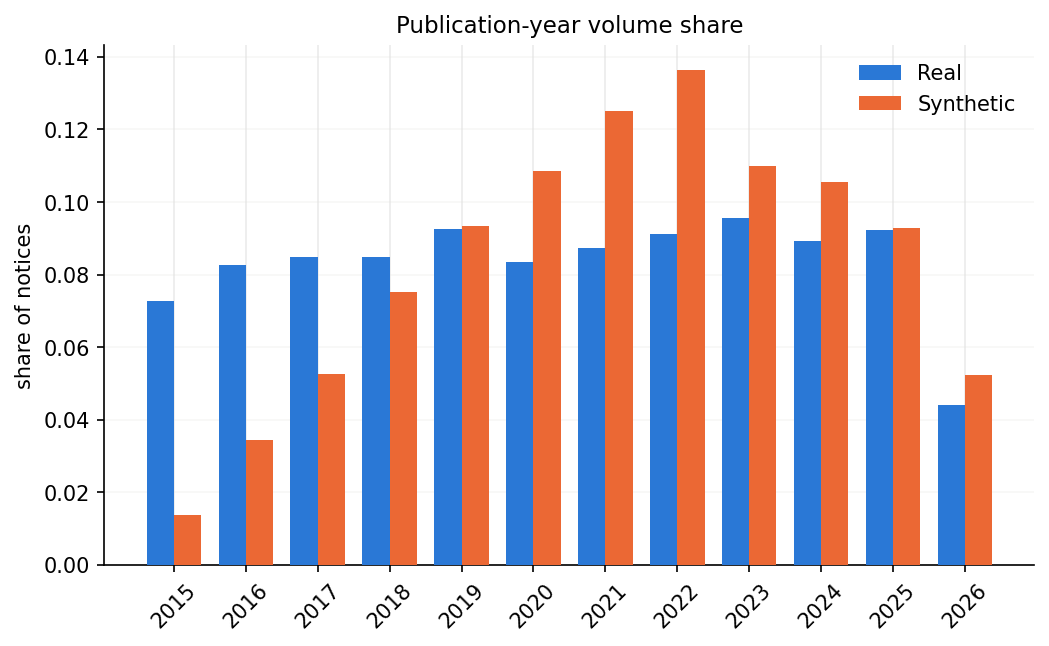
\includegraphics[width=0.86\textwidth]{synthetic_benchmark/v0_2_conditional_revision/temporal_year_share_real_vs_synthetic.png}
\caption{Publication-year composition. This visual checks whether synthetic notices are spread across years similarly to the real corpus. It is a calendar-structure check, not a linkage-accuracy check.}
\label{fig:year-share}
\end{figure}

\begin{figure}[h!]
\centering
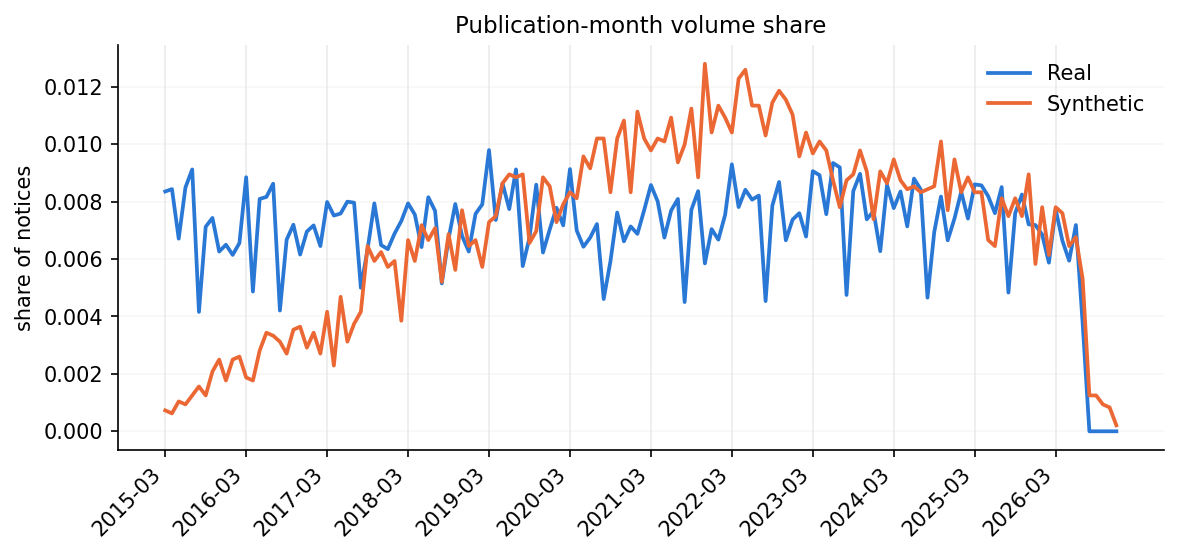
\includegraphics[width=0.86\textwidth]{synthetic_benchmark/v0_2_conditional_revision/temporal_month_share_real_vs_synthetic.png}
\caption{Publication-month composition. This supports the seasonal/calendar plausibility of the benchmark.}
\label{fig:month-share}
\end{figure}

\begin{figure}[h!]
\centering
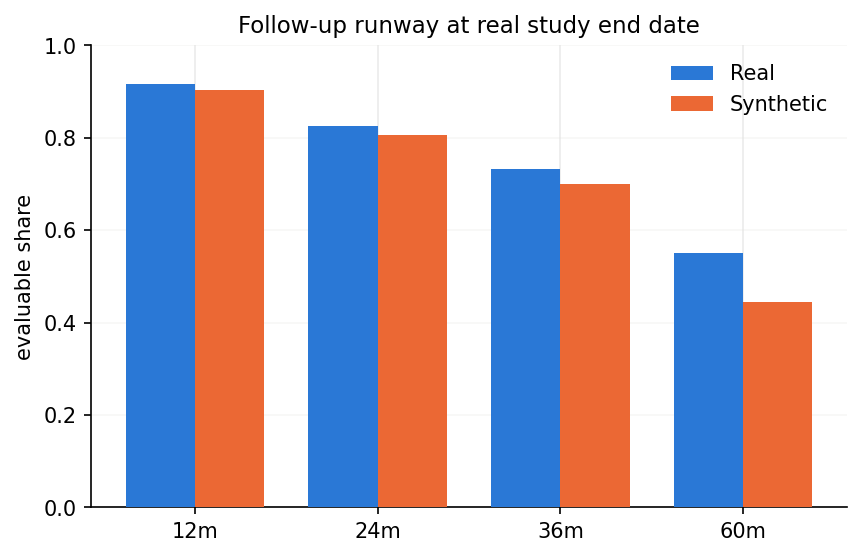
\includegraphics[width=0.86\textwidth]{synthetic_benchmark/v0_2_conditional_revision/temporal_followup_runway_real_vs_synthetic.png}
\caption{Follow-up runway comparison. The 12- and 24-month horizons pass; the 60-month horizon remains visibly weaker and should be stated as a limitation in downstream linkage evaluation.}
\label{fig:followup-runway}
\end{figure}

\subsection{Candidate environment}

\begin{table}[h!]
\centering
\caption{Layer-1 algorithm source-scope candidate environment.}
\begin{tabular}{lrrrrrr}
\toprule
Scope & Sources & Zero-cand. & Mean & p75 & p90 & p95 \\
\midrule
Real & 3,159 & 60.9\% & 1.94 & 2 & 6 & 10 \\
v0.2 synthetic & 354 & 90.4\% & 0.15 & 0 & 0 & 1 \\
v0.3 synthetic & 395 & 63.0\% & 0.64 & 1 & 2 & 3 \\
\bottomrule
\end{tabular}
\end{table}

The key improvement is the zero-candidate rate. In v0.2, most synthetic sources had no possible candidates, so downstream scoring algorithms would mostly be tested on an unrealistically empty environment. In v0.3, the zero-candidate rate is within 2.16 percentage points of the real Layer-1 source scope. The upper candidate-count tail remains lighter than the real corpus, but it passes the predefined p75, p90, and p95 gates.

\begin{figure}[h!]
\centering
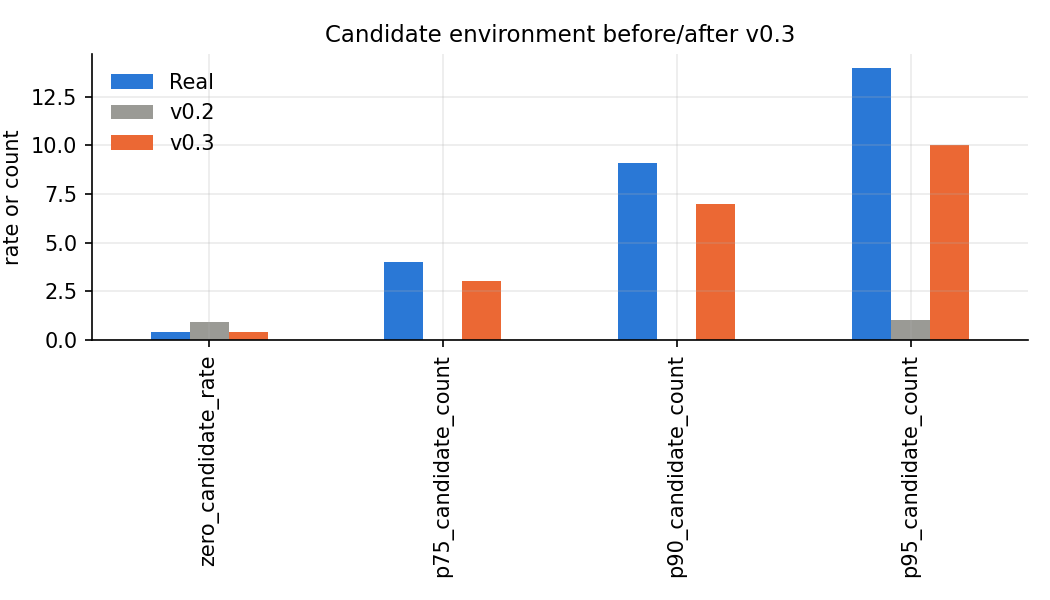
\includegraphics[width=0.88\textwidth]{synthetic_benchmark/v0_3_temporal_candidate_revision/candidate_environment_before_after.png}
\caption{Candidate environment before and after v0.3. This is the most important visual for linkage-readiness: it shows that the actual production candidate generator now sees a realistic enough source/candidate environment.}
\label{fig:candidate-before-after}
\end{figure}

\subsection{Structural truth}

\begin{table}[h!]
\centering
\caption{Structural-truth checks for v0.3.}
\begin{tabular}{lrl}
\toprule
Metric & Value & Status \\
\midrule
Cycles & 6,866 & PASS \\
Successor relation rate & 30.1\% & Diagnostic \\
Share of true gaps over 6 months & 81.2\% & PASS \\
Observed truth columns & 0 & PASS \\
Metadata validation status & PASS & PASS \\
\bottomrule
\end{tabular}
\end{table}

The broad true-gap tail is especially important. A share of 81.2\% of true successor gaps remains above six months, well above the minimum gate of 45\%. This means the revision did not collapse all truth into the production candidate window merely to make the candidate generator look better.

\section{Layered Validation Framework}

The freeze gate described above answers one question: does the synthetic corpus resemble the real corpus on the properties that were checked? A benchmark needs more than that. A generator can reproduce every observable marginal and still encode the wrong latent mechanism, leak truth into the observed table, copy a real record, or present a linkage task that is trivially solvable. These are separate failure modes and no single goodness-of-fit test detects them.

The validation framework therefore runs a matrix of fifteen gates across five layers, implemented in \texttt{src/boamp/synthetic/validation\_framework/} and executed by \nolinkurl{scripts/validate_synthetic_benchmark.py}. Every check writes one row of a machine-readable long table carrying the real estimate, the synthetic estimate, the difference, an effect size, a bootstrap interval where one is available, the predeclared tolerance, and a status.

\subsection{Decision rule}

Statistical non-rejection is not evidence of equivalence. With roughly 87{,}000 real and 9{,}471 synthetic notices, an equality test rejects on differences far too small to matter for linkage; in sparse subgroups it misses differences that matter a great deal. Decisions are therefore made on intervals against practical tolerances rather than on $p$-values.

For a difference parameter $\theta = \theta_S - \theta_R$ and a predeclared bound $\Delta$, the two one-sided tests procedure supports practical equivalence only when the whole interval lies inside $(-\Delta, +\Delta)$. Resampling is clustered at the buyer level, because notices from one buyer share text, identifiers and missingness behaviour, and an i.i.d.\ bootstrap would report intervals several times too narrow. A metric with no interval available can reach at most ``not obviously discrepant'', never ``equivalent''.

Four statuses are used. \textsc{Pass} means the interval lies inside the tolerance or the invariant holds exactly. \textsc{Warning} means the estimate crosses a tolerance, the evidence is too thin to decide, or a non-critical discrepancy remains. \textsc{Fail} means a critical invariant broke, truth leaked, a real record was copied, or a core property is materially outside tolerance. \textsc{Inconclusive} means the check could not be run; it is never read as a pass. The statuses are deliberately not averaged into a single score, because a high average conceals a fatal defect.

\subsection{Gate results}

\begin{table}[h!]
\centering
\caption{Validation gate results for v0.3 \texttt{central\_provisional}. Critical gates block release on their own; non-critical breaches are recorded in the fidelity budget.}
\small
\begin{tabular}{p{0.28\textwidth}p{0.10\textwidth}p{0.08\textwidth}p{0.40\textwidth}}
\toprule
Gate & Status & Critical & Headline finding \\
\midrule
Internal integrity & WARNING & yes & All 31 invariant, leakage, replay and negative-control checks hold; byte-identical regeneration untested. \\
Specification recovery & \textbf{FAIL} & yes & The scenario file does not reproduce the dataset, and the mean true gap falls outside its Monte Carlo interval. \\
Marginals & WARNING & no & Department mix and the duration distribution differ materially. \\
Conditionals & PASS & yes & Conditional field rates within tolerance. \\
Temporal & WARNING & yes & 60-month runway remains the known caveat. \\
Candidate environment & PASS & yes & Zero-candidate rate and percentiles within gates. \\
Missingness (fieldwise) & WARNING & no & \siren{} presence differs by 5.2 pp. \\
Missingness structure & PASS & no & Joint patterns, entropy and co-occurrence lift all within tolerance. \\
Buyer activity & WARNING & no & Activity concentration far too flat (Gini 0.56 vs 0.83). \\
Names and identifiers & WARNING & no & Within-buyer name variation close on a silver standard. \\
Text & WARNING & no & Internal duplication 9.0\% vs real 51.4\%; bigram profile diverges. \\
Privacy and memorisation & PASS & yes & Zero record-specific copies; near-neighbour similarity below the real-vs-real baseline. \\
Hidden-truth difficulty & WARNING & yes & Blocking recovers 36\% of in-scope true matches at the production window. \\
Algorithm utility & PASS & yes & Three probes separate; best pair-F1 0.41. \\
Robustness & WARNING & no & One seed per scenario; seed stability not estimable. \\
\bottomrule
\end{tabular}
\end{table}

\subsection{Internal validity and negative controls}

Internal checks run before any real-versus-synthetic comparison, because a comparison against incoherent truth is meaningless. They cover schema and support, truth-graph consistency (every relation references an existing cycle, exactly one outgoing relation per cycle, successors strictly after their source, acyclic successor graph), count reconciliation across notice, cycle and family grain, leakage isolation, and exact corruption replay: starting from pristine latent values and applying the stored corruption events must reproduce the observed values exactly. All of these hold for v0.3.

The suite also runs five negative controls. Each deliberately breaks a copy of the loaded tables --- leaking a truth column, making a relation self-referential, altering an observed value away from its corruption log, dropping a required column, scrambling membership roles --- and confirms that the corresponding check flips to \textsc{Fail}. Without this, a suite that silently stopped checking anything would report a clean pass forever. All five controls are detected.

\subsection{The specification-recovery failure}

Two parameter-recovery checks fail, and together they identify a genuine defect rather than a bad draw.

First, the v0.3 candidate sweep enables the scoped-candidate block \emph{in memory} and records its chosen parameters in \texttt{generation\_metadata.json}. Loading \texttt{central\_provisional.yaml} and re-running the generator does not reproduce this benchmark. Until the selected parameters are written back into a versioned scenario file, the run manifest is the only complete record of how the data was made.

Second, the realized mean true gap is 15.75 months against a 99\% Monte Carlo interval of $[16.29, 17.31]$ simulated from the effective mixture. The reference correctly accounts for the observation window: a successor exists only if its start still falls inside the window, so the surviving gaps are right-censored by the headroom remaining to each source cycle, and simulating the unconditional draw would fail for reasons unrelated to the generator. The residual discrepancy is attributable to the hard-negative chain alignment in \texttt{cycles.py}, which relocates whole chains near a source's expected end and is not expressible in the saved parameter set.

\subsection{Benchmark difficulty and algorithm utility}

These checks require the sealed truth tables and cannot be computed on real \boamp{} at all. Recall is measured against true matches whose two notices both lie inside the candidate-generation scope, since successors outside it are unreachable by any method operating on these candidates; that scoping loss is reported separately.

Of 2{,}066 true successor pairs in the benchmark, 152 have both notices inside the 395-notice digital candidate scope. At the production six-month window, blocking recovers 36.2\% of them; widening the probe window to 36 months raises this only to 57.9\%. The first figure is a property of that window against this benchmark's renewal gaps and is expected by design, since the gap distribution is deliberately centred outside it. The second is more informative: even with a generous window, buyer-key blocking cannot reach two of every five in-scope true matches, because the buyer key itself drifts across a renewal.

Three probe linkers with frozen parameters --- a deterministic top-1 rule, a score threshold across all ranks, and a Fellegi--Sunter log-odds model over three binary field agreements --- are run to test whether the benchmark discriminates between substantively different methods. None of them is the production acceptance threshold: a pipeline threshold is an output of that pipeline, never a definition of truth. They reach pair-F1 of 0.413, 0.394 and 0.366 respectively. The spread confirms the benchmark separates methods; the ceiling confirms no shortcut solves it; the score overlap between true matches and hard negatives, 0.21, confirms that distinguishing them requires real discrimination rather than a threshold on an obvious gap.

\subsection{Privacy and memorisation}

The generator was built from calibrated aggregate statistics rather than fitted to row-level \boamp{}, but this is verified rather than assumed. No synthetic procurement object reproduces a real one outside the generator's own declared template pools. Near-copy risk is assessed against a baseline instead of against zero: five-token shingle Jaccard similarity to the nearest real text has a synthetic p95 of 0.043 against a real-versus-real holdout baseline of 0.807, so synthetic text sits far further from real text than real texts sit from each other. Membership-inference auditing remains out of scope and is reported as such, not as a pass.

\subsection{New findings the earlier gates did not surface}

Three material discrepancies were invisible to the freeze gate and are now recorded in the discrepancy register.

\textbf{Buyer activity is far too flat.} Real activity has a Gini coefficient of 0.83 and the top 5\% of buyers hold 66\% of all notices; the synthetic corpus reaches 0.56 and 37\%. This is not a corpus-size artifact --- raw counts are confounded by the benchmark being smaller, so the gate uses activity relative to each corpus's own mean, and the gap persists. Concentration determines how dense candidate neighbourhoods become, so this understates the difficulty of the most demanding linkage cases.

\textbf{Internal text duplication collapsed.} Real \boamp{} objects are non-unique 51.4\% of the time; the synthetic corpus reaches 9.0\%. The v0.1 calibration explicitly targeted and hit this quantity, so the v0.2 conditional-reuse revision --- which replaced the global boilerplate rate --- appears to have regressed it. Because text is what a linker falls back on when identifiers are weak, a corpus whose texts are too distinctive makes linkage easier than it really is.

\textbf{The duration tail is wrong at p99.} The freeze gate checked duration presence, not its distribution. Real p99 declared duration is 72 months against a synthetic 360.

\section{Why the Benchmark Is Ready for Linkage Algorithms}

The benchmark is ready because the validation evidence now matches the task the linkage algorithms will face. Earlier versions could match some global or conditional field statistics but still fail to produce a realistic candidate environment. That is not sufficient: a linkage algorithm first needs plausible candidates before scoring can matter.

The v0.3 benchmark passes the hard readiness gates:
\begin{itemize}
    \item observed field availability and text reuse are close to real conditional patterns;
    \item temporal notice distribution is close enough for the planned evaluation stage;
    \item the actual Layer-1 candidate generator produces a realistic enough zero-candidate rate and candidate-count distribution;
    \item hidden truth exists, is internally coherent, and is not present in the observed notices;
    \item v0.3 did not use linkage thresholds or accepted links as tuning targets.
\end{itemize}

Therefore, the next valid step is to run the linkage algorithms on \texttt{observed\_notices.parquet}, produce predicted links, and only then compare those predictions against \texttt{true\_relations.parquet}. Linkage-score calibration, threshold optimization, and precision/recall interpretation belong to that next stage, not to the benchmark-generation stage.

The layered validation framework sharpens what ``ready'' means here, and narrows it. The framework confirms the two properties that would otherwise invalidate every downstream number: hidden truth is internally coherent and does not leak, and no real record has been copied. It also confirms that the task is worth running --- three substantively different probe linkers separate from one another, none of them solves the benchmark, and true matches genuinely overlap with hard negatives in score space.

What it does not yet support is a defensible \emph{final ranking} of linkage algorithms. The current saved scenario parameters reproduce the central dataset, the validation run performs canonical replay, and the all-artifact replay audit passes for 51 generated artifacts. Ten seeds now exist for the central scenario and for each required easier/moderate/difficult/stress scenario. However, headline difficulty remains scenario-dependent and the probe-linker rankings are unstable within scenarios and across scenario means. Accordingly, the five-level readiness assessment is authoritative: \texttt{PIPELINE\_TECHNICALLY\_VALID}, \texttt{READY\_FOR\_PRELIMINARY\_MODELING}, and \texttt{READY\_FOR\_CONTROLLED\_ALGORITHM\_COMPARISON} pass with limitations, while \texttt{READY\_FOR\_FINAL\_ALGORITHM\_RANKING} and \texttt{READY\_FOR\_VALIDATED\_SYNTHETIC\_BENCHMARK\_RELEASE} fail.

\section{Limitations and Caveats}

The benchmark has passed the current readiness gate, but several limitations remain.
\begin{enumerate}
    \item \textbf{Synthetic evidence is not real legal truth.} It can test whether an algorithm behaves sensibly in a controlled realistic environment, but it cannot prove real-world renewal accuracy.
    \item \textbf{Some latent quantities are scenario assumptions.} Recurrence prevalence, broad successor-gap distribution, and text drift are documented assumptions where real truth is unavailable.
    \item \textbf{The 60-month follow-up runway is weaker.} The 12- and 24-month gates pass, but the 60-month comparison remains a caveat.
    \item \textbf{Candidate upper tail remains lighter than real.} The candidate-environment gate passes, but the real p90 and p95 candidate counts remain higher than the central synthetic values.
    \item \textbf{No score calibration has been done yet.} The benchmark is ready only for controlled synthetic comparisons with limitations, not for claiming final linkage performance.
    \item \textbf{The current worktree is not release-clean.} \texttt{source\_state\_manifest.json} hashes the dirty source/artifact state, \texttt{dirty\_state\_overlay.tar.gz} packages that overlay against the recorded Git HEAD, and \texttt{dirty\_state\_overlay\_verification.json} verifies replay onto a clean Git HEAD snapshot. A release still requires a clean commit or standalone release package.
    \item \textbf{Observable fidelity warnings remain.} Buyer-activity concentration, text lexical distance, identifier completeness, and follow-up-runway warnings remain visible in the discrepancy register and validation manifest.
    \item \textbf{Identifier persistence is a documented trade-off.} A tested notice-type split of family-level identifier persistence reduced one attribution-specific mismatch but introduced a critical conditional text failure and degraded widened blocking reachability. The current generator therefore retains family/need-level identifier persistence.
    \item \textbf{Probe ranking is unstable.} Ten seeds exist for the central and required benchmark scenarios, but probe-linker Kendall-\(\tau\) diagnostics warn within scenarios and across scenario means. This blocks final algorithm-ranking claims.
    \item \textbf{Parts of the specification remain untested.} Byte-identical regeneration, membership-inference risk, neural-embedding semantic distances, Sobol sensitivity analysis, and a held-out real partition never used during generator design are all out of scope. They are reported as not run, never as passed.
\end{enumerate}

\section{Reproducibility and Source Inventory}

The main notebook for the final validation is
\nolinkurl{notebooks/10_synthetic_temporal_candidate_revision_validation.ipynb}.
The concise generated report is
\nolinkurl{reports/generated/synthetic_benchmark/v0_3_temporal_candidate_revision_report.md}.
The final machine-readable readiness assessment is
\nolinkurl{reports/tables/synthetic_benchmark/v0_3_temporal_candidate_revision/readiness/readiness_decisions.json}.
The selected parameter provenance is
\nolinkurl{reports/tables/synthetic_benchmark/v0_3_temporal_candidate_revision/candidate_revision_selected_parameters.csv}.
The dirty-state overlay archive and its external hash manifest are
\nolinkurl{reports/tables/synthetic_benchmark/v0_3_temporal_candidate_revision/dirty_state_overlay.tar.gz}
and
\nolinkurl{reports/tables/synthetic_benchmark/v0_3_temporal_candidate_revision/dirty_state_overlay_manifest.json};
the replay verification is
\nolinkurl{reports/tables/synthetic_benchmark/v0_3_temporal_candidate_revision/dirty_state_overlay_verification.json}.
These are audit artifacts, not final-release approval.

The layered validation framework is documented by the data-generating-process specification at
\nolinkurl{docs/synthetic_benchmark_dgp_specification.md}
and summarised by
\nolinkurl{notebooks/12_synthetic_validation_framework_summary.ipynb}.
It is executed by
\nolinkurl{scripts/validate_synthetic_benchmark.py},
which writes the metric long table, gate summary, discrepancy register, probe-linker results and run manifest to
\nolinkurl{reports/tables/synthetic_benchmark/v0_3_temporal_candidate_revision/validation_framework/}.
The frozen Phase~0 registries --- data dictionary, unit-of-analysis table, parameter registry with provenance classes, predeclared tolerance registry, and scenario manifest --- are generated by
\nolinkurl{scripts/build_benchmark_registries.py}
into the sibling \texttt{registries/} directory. Both are generated from the code and config that drive generation and validation, so a renamed column or a retuned tolerance appears in the registry on the next run instead of silently diverging from it.

The primary implementation modules reviewed for this report are:
\begin{itemize}
    \item \texttt{src/boamp/synthetic/buyers.py};
    \item \texttt{src/boamp/synthetic/needs.py};
    \item \texttt{src/boamp/synthetic/cycles.py};
    \item \texttt{src/boamp/synthetic/notices.py};
    \item \texttt{src/boamp/synthetic/corruption.py};
    \item \texttt{src/boamp/synthetic/conditional\_observation.py};
    \item \texttt{scripts/generate\_synthetic\_benchmark\_v0\_3\_temporal\_candidate\_revision.py}.
\end{itemize}

\section{Recommended Next Step}

The correct next step is to run linkage algorithms against the v0.3 observed synthetic notices inside labelled scenarios, store their predicted links, and evaluate them against the hidden truth relations. The evaluation should report candidate coverage, ranking quality, precision/recall against hidden truth, threshold sensitivity, seed intervals, scenario sensitivity, and failure cases by buyer-key type, \cpv{} division, text pattern, and temporal gap.

Before that evaluation can support final algorithm \emph{rankings}, three things should be fixed or explicitly bounded. First, demonstrate that algorithm rankings are stable within the intended scenario and under the required scenario envelope, or else report rankings only scenario by scenario. Second, decide whether the remaining observable warnings, especially buyer activity, text lexical distance, identifier completeness, follow-up runway, and candidate upper tail, are scientifically acceptable for the intended comparison. Third, commit or otherwise package the exact source/artifact state so release users can identify the evaluated benchmark immutably.

Until that evaluation is complete, the defensible claim is:
\begin{quote}
Within declared observable tolerances and a documented scenario envelope, the synthetic benchmark reproduces selected \boamp{} structures and candidate difficulties; its hidden truth is internally coherent, does not leak, contains no copied real records, and replays exactly across 51 generated artifacts; and conclusions about linkage algorithms must still be reported with sensitivity to scenario assumptions, seed variation, remaining observable warnings, and the unknown real \boamp{} recurrence truth.
\end{quote}

\end{document}
